%% ======================================================================
%% Journal version — Cross-Domain Synthetic Pre-Training in QCL
%% Draft v0.1 (2026-09-18). Internal working copy, not for submission yet.
%%
%% Status of data: five-seed campaign of the QAI version, statistically
%% re-analysed and with the Experiment-2 mislabelling corrected. Sections
%% marked with %% [PENDING] carry numbers that the 20-seed re-run and the
%% added baselines (EWC, rehearsal, learning-rate control) will replace
%% before submission.
%% ======================================================================
\documentclass[preprint,number,sort&compress]{elsarticle}

\let\Bbbk\relax
\usepackage[T1]{fontenc}
\usepackage{amsmath,amssymb,amsfonts}
\usepackage{graphicx}
\usepackage{textcomp}
\usepackage{xcolor}
\usepackage{booktabs}
\usepackage{multirow}
\usepackage{braket}
\usepackage{pgfplots}
\pgfplotsset{compat=1.17}
\usepackage[linesnumbered,ruled,vlined]{algorithm2e}
\usepackage[hidelinks]{hyperref}

\begin{document}

\begin{frontmatter}

\title{Cross-Domain Synthetic Pre-Training in Quantum Continual Learning: An Empirical Characterisation}

\author[upo]{D. Mart\'in-P\'erez\corref{cor1}}
\ead{dmarper2@upo.es}
\author[upo]{F. Rodr\'iguez-D\'iaz}
\ead{froddia@upo.es}
\author[us]{D. Guti\'errez-Avil\'es}
\ead{dgutierrez3@us.es}
\author[upo]{A. Troncoso}
\ead{atrolor@upo.es}
\author[upo]{F. Mart\'inez-\'Alvarez}
\ead{fmaralv@upo.es}

\cortext[cor1]{Corresponding author}

\address[upo]{Data Science and Big Data Lab, Pablo de Olavide University, ES-41013 Seville, Spain}
\address[us]{Department of Computer Science, University of Seville, ES-41012 Seville, Spain}

\begin{abstract}
Sequential training of variational quantum classifiers produces interference
between tasks, a failure mode known as catastrophic forgetting. Memory-based
remedies conflict with the resource constraints of near-term quantum devices,
which motivates initialisation strategies that leave no memory footprint after
training. This study characterises one such strategy, where a hybrid
classical-quantum model is pre-trained on a synthetic Gaussian source that
shares no semantic content with the target sequence, and the resulting
parameters are transferred to the sequential phase. Five random seeds and
three noise profiles, from an ideal state-vector simulation to a legacy
device-level error budget, support the analysis, and every comparison is
reported with paired tests, effect sizes and bootstrap confidence intervals.
The synthetic prior reduces the forgetting drop of the first task by 7.0 to
9.3 percentage points across the noise profiles, an improvement that reaches
the 0.05 significance level under the calibrated device profile and becomes
unambiguous when the profiles are pooled. A corrected reading of the topology
comparison shows that the architectures with the largest capacity learn the
first task best and also lose the most, while the most constrained
architecture retains more only because it never learns the task well. A
preliminary mechanism analysis based on gradient statistics suggests that the
synthetic prior places the circuit in a region of the optimisation landscape
with substantially stronger gradient signal than random initialisation. The
results are framed as an empirical characterisation, not as a new method, and
the limitations of the current scale are stated explicitly.
\end{abstract}

\begin{keyword}
quantum machine learning \sep continual learning \sep catastrophic forgetting \sep
variational quantum circuits \sep transfer learning
\end{keyword}

\end{frontmatter}

% ======================================================================
\section{Introduction}
% ======================================================================

Variational quantum circuits have become the workhorse of quantum machine
learning in the noisy intermediate-scale quantum regime, where the reliable
circuit size is limited by gate and readout errors \cite{Preskill18,
cerezo2021variational}. A variational circuit encodes classical data into a
quantum state and updates rotation angles through a classical optimiser
\cite{Mitarai18, biamonte2017quantum}, which makes the resulting
model a candidate for classification tasks in settings where the data
arrives as a stream rather than as a single static dataset
\cite{RODRIGUEZ-DIAZ26}. When such a circuit is trained on a sequence of
tasks without access to previous data, the updates for a new task overwrite
the parameters that encoded earlier tasks, and the accuracy on the earlier
tasks collapses. This phenomenon, catastrophic forgetting, has been
characterised in classical networks \cite{McCloskey89,
parisi2019continual} and has recently been observed on superconducting
hardware for quantum classifiers \cite{Zhang26}.

These limits have motivated two families of remedies in the classical
literature. Regularisation-based methods penalise changes to parameters that
were important for previous tasks, with elastic weight consolidation as the
canonical example \cite{kirkpatrick2017overcoming} and with alternatives
that estimate importance online \cite{Zenke17}. Replay-based
methods interleave stored samples or stored predictions with the current
task, from plain experience replay \cite{lopezpaz2017gem} to the
logit-distillation variants that preserve the soft decision boundaries of
previous tasks \cite{buzzega2020dark}. Both families carry costs that sit
badly with the constraints of near-term quantum devices. Regularisation
requires a Fisher information estimate whose storage and computation grow
with the number of parameters, and replay requires a memory buffer whose
size grows with the sequence \cite{mcclean2018barren, Wang21}. Recent
work has shown that replay can be transferred to quantum-classical heads
without destabilising training \cite{martinperez2026derpp}, which raises the
question of what can be done when even a small buffer is not affordable.

In parallel, quantum transfer learning has developed the machinery to reuse
knowledge across domains: a frozen classical network extracts compact
features and a variational circuit is fine-tuned on them, which allows small
quantum circuits to operate on high-dimensional inputs \cite{mari2020transfer,
martinperez2026cmes, martinperez2026soco}. The transfer-learning literature
in the classical setting has long recognised that pre-training on data
unrelated to the target domain still produces features that transfer well
\cite{Yosinski14, pan2009survey}. Whether the same logic holds
for a variational circuit in a sequential setting, and what property of the
resulting initialisation protects later tasks, remains open. The observation
that layerwise initialisation strategies stabilise the training of quantum
circuits \cite{Skolik21} indicates that the starting point of a
variational circuit is not a neutral design choice.

These constraints frame the question of this study: does pre-training a
hybrid quantum-classical classifier on a synthetic source that shares no
semantic content with the target tasks produce an initialisation that
reduces forgetting during later sequential training, and under which
conditions does the effect hold? The present study addresses the question
for a four-qubit hybrid model across three circuit topologies and three noise
profiles, with a statistical protocol built on paired comparisons over seeds.
The contributions are the following. First, the cross-domain synthetic
pre-training setup is formalised for a sequential quantum classifier, with
the source, the task sequence and the evaluation protocol stated precisely.
Second, the comparative evaluation is reported with absolute accuracies,
paired tests, effect sizes and confidence intervals, which corrects two
reporting defects of the earlier conference version of this study, namely
the omission of absolute accuracies and a mislabelled retention table.
Third, a corrected reading of the topology comparison is established, where
the apparently best-retaining architecture is the one with the least
capacity. Fourth, first mechanism evidence is provided, through gradient
variance and landscape probes, for why a synthetic prior changes the
training dynamics of the circuit. The rest of the manuscript is organised as
follows. Section~\ref{sec:related} reviews the related literature.
Section~\ref{sec:background} fixes the scenario definitions and the metrics.
Section~\ref{sec:methodology} describes the pre-training methodology, the
circuit architectures and the sequential protocol.
Section~\ref{sec:setup} details the experimental setup.
Section~\ref{sec:results} reports the results, and
Section~\ref{sec:discussion} discusses their scope and limitations.

% ======================================================================
\section{Related Work}
\label{sec:related}
% ======================================================================

\subsection{Continual learning in classical networks}

The sequential-learning problem was formalised by
McCloskey and Cohen \cite{McCloskey89} and has since produced
a taxonomy of strategies that spans regularisation, replay and architectural
design \cite{parisi2019continual, Lange22, Wang24}. Elastic weight
consolidation introduces a quadratic penalty weighted by the diagonal of the
Fisher information matrix \cite{kirkpatrick2017overcoming}, and synaptic
intelligence replaces the Fisher estimate with an online accumulation of
parameter importance \cite{Zenke17}. Replay-based approaches
store a small subset of previous samples and constrain the updates with
them \cite{lopezpaz2017gem}, and their distillation variants retain the soft
outputs of the model on previous tasks \cite{buzzega2020dark, Li18}. The
distinction between task-incremental, domain-incremental and
class-incremental scenarios \cite{Ven22} is central for the present study,
because strategies that work under a task oracle do not transfer
automatically to settings where the task identity is unknown at inference
time. Parameter-space regularisation has been examined for quantum circuits
\cite{martinperez2026derpp}, while the initialisation of the model, which is
the variable manipulated here, has received less attention in that setting.

\subsection{Quantum transfer learning and quantum continual learning}

Hybrid classical-quantum transfer learning freezes a pre-trained classical
network and trains a variational circuit on its features,
\cite{mari2020transfer}. Extensions of this template have characterised the
effect of device noise \cite{martinperez2026cmes} and the behaviour of
different classical backbones \cite{martinperez2026soco}. Trained
variational circuits are known to suffer from trainability problems, from
barren plateaus in deep circuits \cite{mcclean2018barren, cerezo2021cost,
Sharma22} to noise-induced flattening of the landscape
\cite{Wang21}, and architectures with local connectivity have been
shown to avoid part of these effects \cite{pesah2021absence}. The continual
case is more recent. A regularisation-based quantum continual learning
protocol has been reported on a superconducting processor, where an
elastic-weight-consolidation penalty allowed a quantum classifier to retain
knowledge across three sequential tasks \cite{Zhang26}. Earlier work
described unitary update rules for quantum continual learning in simulation
\cite{senicourt2021quantum}. Across these studies, the pre-training domain
is treated as given, and the question of how the initialisation itself
shapes sequential retention is not isolated.

\subsection{Research gaps}

Table~\ref{tab:comparison} places the present study next to representative
prior work across the dimensions that matter for this analysis. Classical
benchmarks report forgetting under full-data regimes, quantum studies focus
on single-task transfer or on regularisation, and the hardware realisation
of quantum continual learning covers a short sequence with a regularisation
penalty. No prior study isolates the effect of a synthetic cross-domain
initialisation on sequential quantum classifiers, and none reports the
comparison with paired statistics over seeds and per-seed confidence
intervals. These two elements define the space of this study.

\begin{table*}[ht]
\centering
\caption{Positioning against representative prior work. The four rightmost
columns mark, respectively, whether the study reports hardware execution,
more than one random seed, inferential statistics, and a scenario analysis
beyond task-incremental evaluation. Dashes indicate aspects that do not
apply to the study.}
\label{tab:comparison}
\setlength{\tabcolsep}{5pt}
\begin{tabular}{llllccc c}
\toprule
Study & Setting & Mechanism & Sequence & HW & Seeds & Stats & Scenario \\
\midrule
Kirkpatrick et al. \cite{kirkpatrick2017overcoming} & Classical & EWC & Multi & -- & ~ & -- & TIL \\
Buzzega et al. \cite{buzzega2020dark} & Classical & DER++ & Multi & -- & ~ & -- & TIL/CIL \\
Mari et al. \cite{mari2020transfer} & Hybrid & QTL & Single & -- & -- & -- & -- \\
Zhang et al. \cite{Zhang26} & Quantum & EWC & 3 tasks & yes & -- & -- & TIL \\
Mart\'in-P\'erez et al. \cite{martinperez2026derpp} & Hybrid & Replay & Multi & -- & yes & yes & TIL \\
This study & Hybrid & Synthetic prior & 2 tasks & -- & yes & yes & TIL \\
\bottomrule
\end{tabular}
\end{table*}

% ======================================================================
\section{Background and Problem Formulation}
\label{sec:background}
% ======================================================================

\subsection{Variational quantum classifiers}

A variational quantum circuit prepares a state $\ket{\psi(x,\theta)}$ by
applying an encoding unitary that depends on the input $x$ followed by a
parameterised unitary $U(\theta)$, and produces predictions from the
expectation values of a set of observables. Training minimizes a classical
loss with respect to $\theta$ through the parameter-shift rule
\cite{Mitarai18} or through differentiable simulation. The
expressibility and the entangling capability of the parameterised unitary
depend on its topology \cite{sim2019expressibility, grant2018hierarchical},
and the trainability of the circuit depends on the same design choices
\cite{mcclean2018barren, pesah2021absence}.

\subsection{Continual learning scenarios and metrics}

A model that faces a sequence of tasks $\{\mathcal{T}_1, \dots, \mathcal{T}_T\}$
observes the training data of task $t$ while training on task $t$ and, in the
strictest form of the problem, keeps no access to the data of previous
tasks. Two scenarios are distinguished after van de Ven et
al.~\cite{Ven22}. In task-incremental learning the task identity is known at
test time and a shared head evaluates the corresponding decision boundary.
In class-incremental learning the task identity is unknown and a single
output layer must separate classes drawn from every task seen so far. The
present study evaluates the task-incremental scenario and the analysis of
class-incremental behaviour is left to the extended protocol described in
Section~\ref{sec:discussion}.

The evaluation uses the standard continual-learning metrics
\cite{lopezpaz2017gem, Lange22}. Let $A_{t,j}$ be the test accuracy on task
$j$ measured after training through task $t$. The average accuracy and the
average forgetting over the sequence are
\begin{equation}
  \mathrm{AA} = \frac{1}{T}\sum_{j=1}^{T} A_{T,j}, \qquad
  \mathrm{AF} = \frac{1}{T-1}\sum_{j=1}^{T-1} \bigl(\max_{t \leq T} A_{t,j} - A_{T,j}\bigr),
  \label{eq:aa_af}
\end{equation}
and the backward transfer is the signed change of each task accuracy between
its completion and the end of the sequence,
\begin{equation}
  \mathrm{BWT} = \frac{1}{T-1}\sum_{j=1}^{T-1} \bigl(A_{T,j} - A_{j,j}\bigr).
  \label{eq:bwt}
\end{equation}
For the two-task protocol analysed here, the quantity of interest is the
forgetting drop on the first task
\begin{equation}
  \Delta_A = \mathrm{Acc}_A^{\text{init}} - \mathrm{Acc}_A^{\text{final}},
  \label{eq:delta}
\end{equation}
where $\mathrm{Acc}_A^{\text{init}}$ is the accuracy on Task A measured at
the end of the Task A phase and $\mathrm{Acc}_A^{\text{final}}$ is the same
accuracy measured after the Task B phase, on the frozen Task A test set. The
relative retention $r_A = \mathrm{Acc}_A^{\text{final}} /
\mathrm{Acc}_A^{\text{init}}$ is reported alongside $\Delta_A$, because the
absolute drop alone rewards classifiers that never learned the first task.

% ======================================================================
\section{Methodology}
\label{sec:methodology}
% ======================================================================

\subsection{Cross-domain synthetic pre-training}

The methodology separates three domains. The source domain $\mathcal{S}$ is
a synthetic binary classification problem generated in four dimensions from
two Gaussian clusters, with no semantic relation to the target tasks. The
sequential domain contains Task A, a binary classification problem built
from two classes of Fashion-MNIST \cite{Xiao17}, and Task B, a binary
problem built from two classes of MNIST \cite{Lecun98}. A hybrid model
consists of a frozen feature extractor and a variational circuit head. For
image tasks, a MobileNetV2 network pre-trained on ImageNet produces a
feature vector that is reduced to four components by principal component
analysis \cite{Sandler18, pearson1901lines}. For the synthetic source the
four features are drawn directly from the Gaussian generator. All features
are rescaled to the interval $[0, \pi]$ to match the rotation domain of the
encoding layer.

Pre-training minimises the cross-entropy loss of the hybrid model on the
synthetic source for a fixed number of epochs and stores the resulting
parameters $\theta_0$. The sequential phase initialises the circuit with
$\theta_0$ and trains on Task A and then on Task B, as summarised in
Algorithm~\ref{alg:protocol}. Two initialisation references complete the
design: a scratch model, initialised at random, and a cross-domain model
whose source features come from CIFAR-10 images passed through the same
MobileNetV2 backbone \cite{krizhevsky2009cifar}, which separates the effect
of the synthetic source from the effect of pre-training on real images.

\begin{algorithm}[ht]
\small
\caption{Cross-domain sequential protocol with synthetic pre-training.}
\label{alg:protocol}
\SetKwInOut{Input}{Input}\SetKwInOut{Output}{Output}
\Input{Source data $D_S$, tasks $\{D_A, D_B\}$, learning rates $\eta_S, \eta_A, \eta_B$, epochs $E_S, E_A, E_B$}
\Output{$\theta_0$, accuracies $\{\mathrm{Acc}_A^{\text{init}}, \mathrm{Acc}_B, \mathrm{Acc}_A^{\text{final}}\}$, forgetting drop $\Delta_A$}
Sample $\theta$ at random or load a pre-trained initialisation \;
\If{pre-training}{
  Train the hybrid model on $D_S$ with learning rate $\eta_S$ for $E_S$ epochs \;
  Store $\theta_0 \leftarrow \theta$ \;}
Train the model with initialisation $\theta$ on $D_A$ with $\eta_A$ for $E_A$ epochs \;
Evaluate $\mathrm{Acc}_A^{\text{init}}$ on the Task A test set \;
Train the same model on $D_B$ with $\eta_B$ for $E_B$ epochs \;
Evaluate $\mathrm{Acc}_B$ on the Task B test set and $\mathrm{Acc}_A^{\text{final}}$ on the Task A test set \;
Return $\Delta_A = \mathrm{Acc}_A^{\text{init}} - \mathrm{Acc}_A^{\text{final}}$ \;
\end{algorithm}

\subsection{Circuit architectures}

Three topologies are evaluated on four qubits, all preceded by the same
encoding block and followed by the same readout. The encoding applies a
single-qubit rotation around the $X$ axis to each wire,
\begin{equation}
  \ket{\psi_{\text{in}}(x)} = \bigotimes_{i=0}^{n-1} R_X(x_i)\ket{0},
  \label{eq:encoding}
\end{equation}
where $x \in [0,\pi]^{n}$ and $n=4$. The readout measures the expectation of
the Pauli-$Z$ operator on the first two wires,
\begin{equation}
  z_k = \braket{\psi_{\text{out}}}{Z_k}{\psi_{\text{out}}}, \quad k \in \{0, 1\},
  \label{eq:readout}
\end{equation}
with $\ket{\psi_{\text{out}}} = U(\theta)\ket{\psi_{\text{in}}(x)}$. The two
expectation values feed a fully connected classical layer that produces the
binary logits $\hat{y} = Wz + b$, with $W \in \mathbb{R}^{2\times 2}$ and
$b \in \mathbb{R}^{2}$, and the model is trained with categorical
cross-entropy.

\emph{Strongly entangling layers (SEL).} Each layer applies a general
single-qubit rotation $R(\alpha, \beta, \gamma)$ to every wire, followed by a
shifted ring of CNOT gates whose range depends on the layer index,
\begin{equation}
  U_{\text{SEL}}(\theta) = \prod_{\ell=1}^{L}
  \Bigl[\prod_{q=0}^{n-1} R_q(\theta_{\ell,q,1}, \theta_{\ell,q,2}, \theta_{\ell,q,3}) \cdot
  \prod_{q=0}^{n-1} \mathrm{CNOT}\bigl(q, (q + r_\ell) \bmod n\bigr)\Bigr],
  \label{eq:sel}
\end{equation}
where $r_\ell = (\ell - 1) \bmod (n-1) + 1$ and the parameter tensor has
shape $(L, n, 3)$, which gives $36$ parameters for the configuration used
here.

\emph{Basic entangler (BE).} Each layer applies one rotation around the $X$
axis per wire, followed by a ring of CNOT gates,
\begin{equation}
  U_{\text{BE}}(\theta) = \prod_{\ell=1}^{L}
  \Bigl[\prod_{q=0}^{n-1} R_X(\theta_{\ell,q}) \cdot
  \prod_{q=0}^{n-1} \mathrm{CNOT}\bigl(q, (q+1) \bmod n\bigr)\Bigr],
  \label{eq:be}
\end{equation}
with a parameter tensor of shape $(L, n)$, which gives $12$ parameters.

\emph{Tree tensor network (TTN).} The tree pairs its wires hierarchically.
At the first level, adjacent wires are paired and the information of each
pair accumulates on the right wire, and the procedure repeats on the
surviving wires until a single wire remains. Each block applies one
rotation around $Y$ and one rotation around $Z$ followed by a CNOT,
\begin{equation}
  U_{\text{TTN}}(\theta) = \prod_{\ell=1}^{L} \prod_{b=0}^{n-2}
  \mathrm{CNOT}(i_b \to j_b)\, R_Z(\theta_{\ell,b,2})_{j_b}\, R_Y(\theta_{\ell,b,1})_{i_b},
  \label{eq:ttn}
\end{equation}
where $(i_b, j_b)$ is the wire pair of block $b$ in the hierarchical wiring.
The parameter tensor has shape $(L, n-1, 2)$, which gives $18$ parameters for
$n=4$ and $L=3$. Two properties of this construction are relevant for the
reading of the results. First, the accumulation of information proceeds
towards the right end of the tree, so the subset of parameters that feeds the
first two wires, where the readout of Eq.~(\ref{eq:readout}) is placed, is
smaller than the nominal parameter count. Second, the blocks that act on
subtrees disconnected from the readout wires contribute no gradient under
this readout configuration, an effect measured in the mechanism analysis of
Section~\ref{sec:mechanism}. The comparison across topologies is therefore
also a comparison across effective circuit sizes, and it is reported as such.

\subsection{Sequential training protocol}

The sequential protocol trains a fresh model per configuration and seed. The
pre-training phase runs for fifteen epochs on the source data. The Task A
phase loads the pre-trained parameters $\theta_0$ or a random initialisation
and trains on Task A for ten epochs, after which
$\mathrm{Acc}_A^{\text{init}}$ is evaluated. The Task B phase continues the
training on Task B for ten further epochs with the same optimiser state, and
the protocol ends with the evaluation of $\mathrm{Acc}_B$ and
$\mathrm{Acc}_A^{\text{final}}$. No replay buffer and no parameter-space
penalty are used in the reference protocol. The learning rate differs across
phases and conditions by design of the original campaign, and the
implications of that design choice are discussed with the results.

\subsection{Noise profiles}

Every configuration is replicated under three noise profiles. The ideal
profile propagates the circuit through the state-vector simulator. The two
noisy profiles insert a single-qubit depolarising channel after every
parameterised rotation, a two-qubit depolarising channel after every two-qubit gate, and a bit-flip channel on every measured wire to
emulate readout error. The device profile borrows its parameters from the
median calibration of the IBM Heron r2 generation, with a single-qubit
depolarising rate of $3\times10^{-4}$, a two-qubit rate of $3\times10^{-3}$
and a readout error of $1.5\times10^{-2}$. The legacy profile scales those
rates towards earlier device generations, with a single-qubit rate of
$10^{-3}$, a two-qubit rate of $1.5\times10^{-2}$ and a readout error of
$3\times10^{-2}$.

% ======================================================================
\section{Experimental Setup}
\label{sec:setup}
% ======================================================================

\subsection{Datasets}

Four data sources participate in the pipeline and Table~\ref{tab:datasets}
summarises their splits. The synthetic source generates two Gaussian
clusters in four dimensions with the \texttt{make\_classification} routine of
scikit-learn. Task A uses classes 0 and 1 of Fashion-MNIST \cite{Xiao17} and
Task B uses classes 2 and 3 of MNIST \cite{Lecun98}. The cross-domain
reference extracts MobileNetV2 features from CIFAR-10 classes 2 and 3
\cite{krizhevsky2009cifar, Sandler18} and reduces them to four components.
All image sources are reduced to four principal components fitted on the
training split and rescaled to $[0,\pi]$.

\begin{table}[ht]
\centering
\caption{Sample counts per data source. The synthetic source is drawn
directly in four dimensions. Image sources traverse a frozen MobileNetV2
backbone before the principal-component reduction.}
\label{tab:datasets}
\begin{tabular}{llccc}
\toprule
Source & Role & Train & Test & Classes \\
\midrule
Synthetic (Gaussian clusters) & Source & 2000 & 500 & 2 \\
CIFAR-10 (MobileNetV2 features) & Source reference & 1000 & 200 & 2, 3 \\
Fashion-MNIST & Task A & 1000 & 200 & 0, 1 \\
MNIST & Task B & 1000 & 200 & 2, 3 \\
\bottomrule
\end{tabular}
\end{table}

\subsection{Statistical protocol}

Every configuration is executed with five independent random seeds and every
reported quantity is the mean over seeds with its standard deviation.
Comparisons between two configurations are paired by seed, which removes the
seed-to-seed variance of the shared pipeline from the contrast. Each paired
comparison reports the mean difference, a two-sided paired $t$-test, a
Wilcoxon signed-rank test as a distribution-free check, the Cohen $d_z$
effect size and a 95\% bootstrap confidence interval of the mean difference
estimated with twenty thousand resamples of the seed pairs. Families of
comparisons are corrected with the Holm procedure. The analysis code and the
per-seed payloads are stored with the repository described in the data
availability statement. The reported Wilcoxon probabilities illustrate a
known limitation of five-seed campaigns, namely that the smallest attainable
two-sided $p$-value of the signed-rank test with five pairs is $0.0625$,
which is why the paired $t$-test and the bootstrap interval carry the
inferential weight here and why the extended campaign of
Section~\ref{sec:discussion} raises the seed count.

\subsection{Implementation and resources}

The pipeline is implemented in Python 3.11 with PennyLane 0.44.1 for the
quantum simulation, PyTorch 2.10.0 for the hybrid model and the optimiser,
scikit-learn 1.8.0 for the feature reduction, and NumPy 2.4.3. The ideal
profile runs on the state-vector device with the adjoint differentiation
method and the noisy profiles run on the density-matrix device with
backpropagation. The optimiser is Adam with a batch size of 32 and a
learning rate of 0.05 during pre-training. All experiments run on the
Hercules cluster of the Centro de Inform\'atica Cient\'ifica de Andaluc\'ia,
on standard nodes with four CPU cores and eight gigabytes of memory, as
independent jobs of SLURM arrays. The complete five-seed campaign over the
three noise profiles consists of forty-five sequential trainings per
experiment.

% ======================================================================
\section{Results}
\label{sec:results}
% ======================================================================

\subsection{Experiment 1: does the synthetic prior reduce the drop?}

Table~\ref{tab:exp1} reports the forgetting drop on Task A for the random
initialisation and for the synthetic prior across the three noise profiles,
with the paired reduction and its bootstrap interval. Under the device
profile, the random initialisation loses $72.90 \pm 2.01$ points of Task A
accuracy after the Task B phase, and the synthetic prior reduces the loss to
$65.10 \pm 3.73$ points, a paired reduction of $7.80$ points whose bootstrap
interval $[4.50, 12.30]$ excludes zero and whose paired test arrives at
$p = 0.028$. The ideal profile shows a reduction of $7.00$ points with a
wider interval, and the legacy profile shows the largest nominal reduction,
$9.30$ points, with the widest spread, which reflects the larger seed
variance of the noisiest condition. When the fifteen seed pairs of the three
profiles are pooled, the reduction is $8.03$ points with a bootstrap interval
of $[4.47, 11.63]$, a paired test below $0.001$, a signed-rank test at
$0.003$ and an effect size of $d_z = 1.09$.

\begin{figure}[ht]
\centering
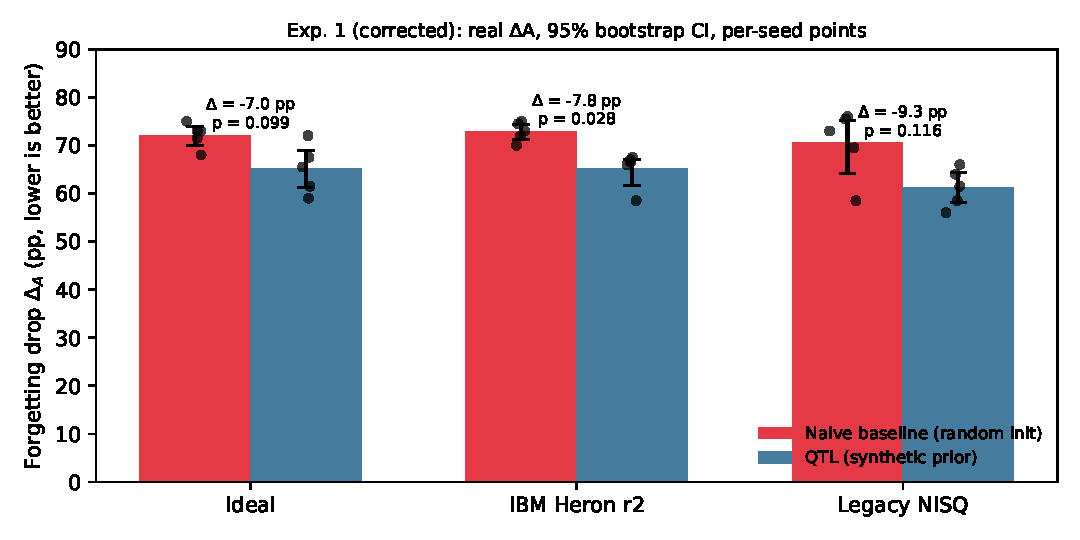
\includegraphics[width=0.85\linewidth]{figures/fig1_exp1_forgetting_corrected.pdf}
\caption{Experiment 1. Forgetting drop on Task A per noise profile for the
random initialisation and the synthetic prior. Bars show the mean over five
seeds, markers show the per-seed values, and whiskers show the 95\% bootstrap
confidence interval of the paired reduction.}
\label{fig:exp1}
\end{figure}

% Corrected Experiment 1 table (Paper 191 revision).
% Values recomputed from results/*/results_seed_*.json (5 seeds per noise profile).
% Columns: mean, bootstrap 95% CI of the drop, paired reduction vs baseline, significance.
\begin{table}[ht]
\centering
\caption{Experiment 1 (corrected). Forgetting drop $\Delta_A$ on Task A, in percentage points (mean $\pm$ std over five seeds), with the paired reduction obtained by synthetic pre-training and its 95\% bootstrap confidence interval. Significance from a two-sided paired $t$-test over seeds (df$=4$); the Wilcoxon signed-rank test cannot reach $p<0.05$ with five seeds. The QTL arm in this experiment runs Task A at $\eta=0.01$ and Task B at $\eta=0.005$, against $\eta=0.05$ for both tasks in the baseline; the reduction therefore mixes the effect of the initialization with the effect of the optimisation regime (see the learning-rate control experiment of the revision).}
\label{tab:exp1}
\begin{tabular}{lcccc}
\toprule
Noise profile & Baseline $\Delta_A$ & QTL $\Delta_A$ & Reduction & $p$ \\
\midrule
Ideal       & $72.10 \pm 2.61$ & $65.10 \pm 5.09$ & $7.00$ [1.10, 12.40] & $0.099$ \\
Heron r2    & $72.90 \pm 2.01$ & $65.10 \pm 3.73$ & $7.80$ [4.50, 12.30] & $0.028$ \\
Legacy NISQ & $70.50 \pm 7.19$ & $61.20 \pm 4.04$ & $9.30$ [0.80, 17.10] & $0.116$ \\
\bottomrule
\end{tabular}
\end{table}


The absolute magnitude of the effect deserves a precise statement. The
reduction corresponds to roughly ten percent of the baseline drop under the
device profile, and the residual loss of about sixty-five points shows that
the synthetic prior delays the interference between tasks without cancelling
it. The learning rate used by the pre-trained arm in this experiment differs
from the rate of the random reference, as the caption of Table~\ref{tab:exp1}
records, so the measured reduction mixes the effect of the initialisation
with the effect of the optimisation regime. The extended protocol repeats
the experiment with matched learning rates and adds regularisation and
replay baselines, and the conclusions of this section are conditional on
that control.

\subsection{Experiment 2: topology capacity and retention}

The second experiment compares the three circuit topologies under the same
sequential load. Table~\ref{tab:exp2} reports, per topology, the Task A
accuracy at the end of the Task A phase, the Task A accuracy at the end of
the Task B phase, the resulting drop, the Task B accuracy and the relative
retention. The corrected reading of this comparison differs from the one
distributed with the conference version of this study, and the difference is
instructive. The architectures with the largest capacity, SEL and TTN, reach
the highest Task A accuracies, $96.5$ and $95.4$ points under the device
profile, and both lose nearly all of that accuracy after the Task B phase,
with retention values of $0.26$ and $0.25$. The basic entangler, whose
single-axis rotations restrict its capacity, reaches only $73.1$ points on
Task A and retains $62.5$ points, a retention of $0.86$. The constrained
topology appears the most stable in relative terms while being the weakest
in absolute terms, since it never expresses the first task well enough to
have much to lose. The paired tests resolve the contrast between the basic
entangler and each of the other two topologies below the $0.001$ level after
Holm correction, while the contrast between SEL and TTN does not reach the
$0.05$ level under any profile. The comparison across topologies is thus a
comparison across effective capacities, which is consistent with the
structural analysis of the readout noted in Section~\ref{sec:methodology}.

\begin{figure}[ht]
\centering
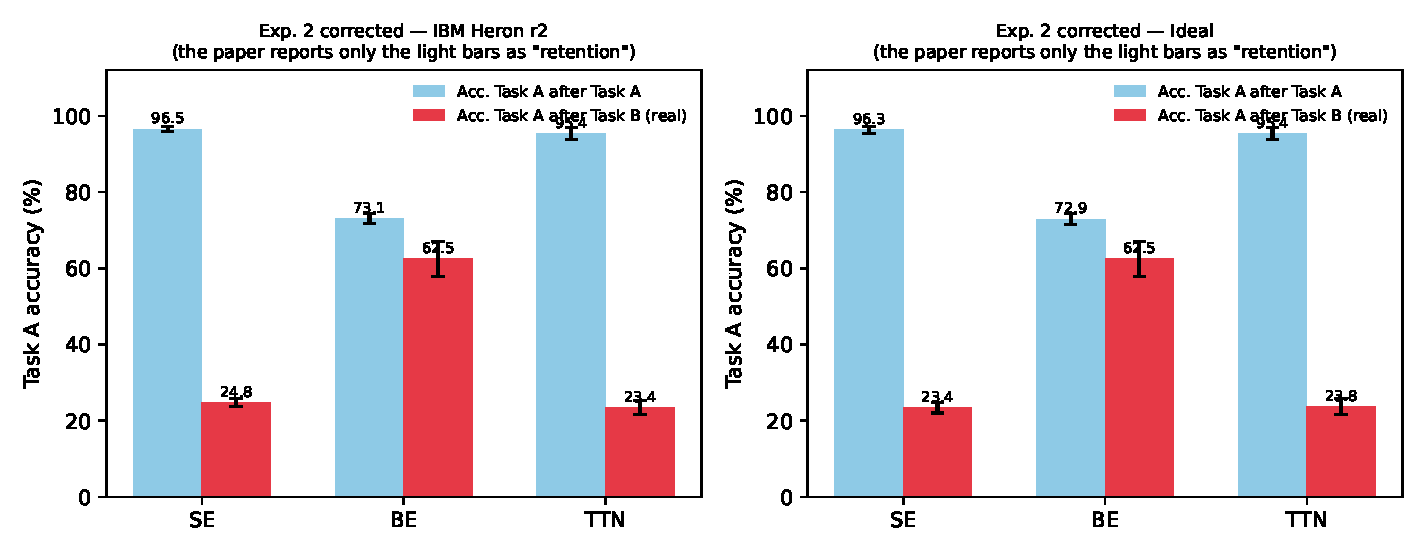
\includegraphics[width=0.85\linewidth]{figures/fig2_exp2_retention_corrected.pdf}
\caption{Experiment 2. Task A accuracy before and after the sequential
exposure to Task B for each topology under the device noise profile. The gap
between the two measurements is the true forgetting drop.}
\label{fig:exp2a}
\end{figure}

\begin{figure}[ht]
\centering
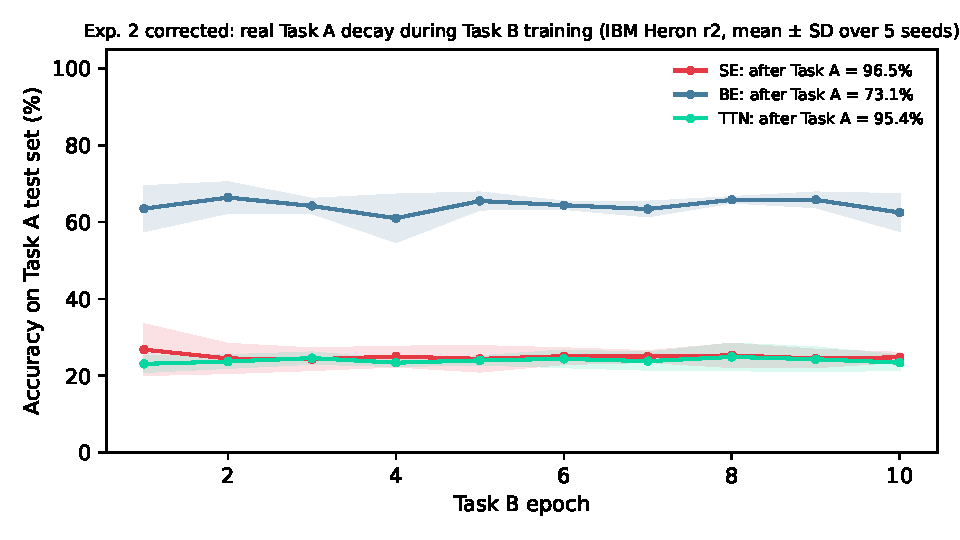
\includegraphics[width=0.85\linewidth]{figures/fig2b_exp2_decay_corrected.pdf}
\caption{Experiment 2. Task A accuracy along the Task B phase for each
topology, mean over five seeds with one standard deviation bands.}
\label{fig:exp2b}
\end{figure}

% Corrected Experiment 2 table (Paper 191 revision).
% Replaces the table whose rows were labelled "final Task A accuracy after Task B"
% while reporting the accuracy measured immediately after Task A training.
% acc_A(init)  = accuracy on Task A after the Task A phase  (JSON field exp2.*.acc_A)
% acc_A(post)  = accuracy on Task A at the last epoch of the Task B phase (exp2.*.acc_history[-1])
\begin{table}[ht]
\centering
\caption{Experiment 2 (corrected). Task A accuracy before and after the sequential exposure to Task B, with the resulting forgetting drop, for the three ans\"atze. Mean $\pm$ std over five seeds. $\mathrm{Acc}_A^{\text{init}}$ is measured at the end of the Task A phase and $\mathrm{Acc}_A^{\text{post}}$ at the end of the Task B phase, on the frozen Task A test set.}
\label{tab:exp2}
\begin{tabular}{llccccc}
\toprule
Noise profile & Ansatz & $\mathrm{Acc}_A^{\text{init}}$ & $\mathrm{Acc}_A^{\text{post}}$ & $\Delta_A$ & $\mathrm{Acc}_B$ & Retention \\
\midrule
\multirow{3}{*}{Ideal}
  & SE  & $96.30 \pm 0.91$ & $23.40 \pm 1.39$ & $72.90$ & $90.20 \pm 1.60$ & $0.24$ \\
  & BE  & $72.90 \pm 1.52$ & $62.50 \pm 4.60$ & $10.40$ & $57.90 \pm 2.33$ & $0.86$ \\
  & TTN & $95.40 \pm 1.56$ & $23.80 \pm 2.08$ & $71.60$ & $90.40 \pm 0.89$ & $0.25$ \\
\midrule
\multirow{3}{*}{Heron r2}
  & SE  & $96.50 \pm 0.61$ & $24.80 \pm 1.04$ & $71.70$ & $89.60 \pm 1.14$ & $0.26$ \\
  & BE  & $73.10 \pm 1.34$ & $62.50 \pm 4.64$ & $10.60$ & $58.20 \pm 2.36$ & $0.86$ \\
  & TTN & $95.40 \pm 1.56$ & $23.40 \pm 1.78$ & $72.00$ & $89.80 \pm 0.67$ & $0.25$ \\
\midrule
\multirow{3}{*}{Legacy NISQ}
  & SE  & $96.70 \pm 0.57$ & $24.60 \pm 3.23$ & $72.10$ & $89.90 \pm 2.27$ & $0.25$ \\
  & BE  & $72.30 \pm 0.91$ & $63.40 \pm 3.23$ & $8.90$  & $58.30 \pm 1.25$ & $0.88$ \\
  & TTN & $95.30 \pm 1.20$ & $22.00 \pm 0.79$ & $73.30$ & $90.60 \pm 0.74$ & $0.23$ \\
\bottomrule
\end{tabular}
\end{table}


\subsection{Experiment 3: convergence under the cross-domain prior}

The third experiment compares three initialisations of the same model on the
MNIST target, a random initialisation, the synthetic prior and the
MobileNetV2 prior, and Table~\ref{tab:exp3} reports the resulting target
accuracies. The three initialisations reach accuracies inside a band of
approximately $1.5$ points, and no paired contrast reaches the $0.05$ level
under any profile. The synthetic prior does not raise the accuracy ceiling
of the target task. The variance across seeds is smaller under the synthetic
prior than under the random initialisation in the device profile, $0.65$
against $1.72$ points, which indicates that the prior stabilises the
outcome without changing its level. The convergence curves in
Figure~\ref{fig:exp3} show that the pre-trained arms start from lower
cross-entropy values and reach the plateau earlier, which is consistent with
the transfer-learning reading of the synthetic source.

\begin{figure}[ht]
\centering
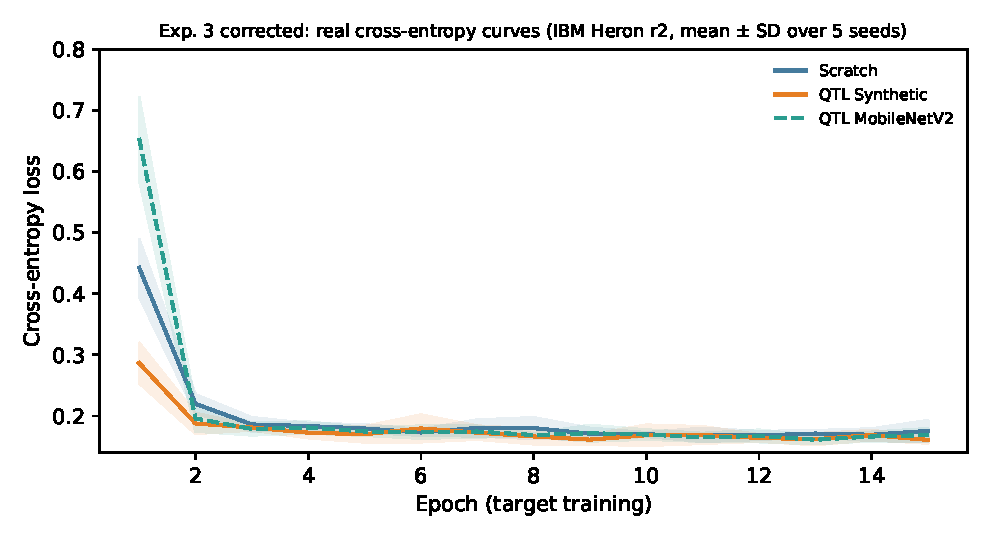
\includegraphics[width=0.85\linewidth]{figures/fig3_exp3_convergence_corrected.pdf}
\caption{Experiment 3. Cross-entropy loss along the target-training epochs
for the three initialisation paradigms under the device noise profile. Lines
show the mean over five seeds and the shaded bands show one standard
deviation.}
\label{fig:exp3}
\end{figure}

% Experiment 3 (journal version).
% Cross-domain initialisation: target (MNIST 2/3) accuracy per initialisation
% paradigm, with the paired contrast against the scratch reference.
% Mean +/- std over five seeds. p-values are Holm-adjusted within the family.
\begin{table}[ht]
\centering
\caption{Experiment 3. Target accuracy (percentage) on the MNIST 2/3 test set
for the three initialisation paradigms, with the paired difference of the
synthetic prior against the scratch reference and its Holm-adjusted
significance from a paired $t$-test over five seeds. No contrast falls below
the 0.05 level in the current five-seed campaign.}
\label{tab:exp3}
\begin{tabular}{lccccc}
\toprule
Noise profile & Scratch & QTL-Syn & QTL-Mob & $\delta$ (Syn--Scr) & $p_\text{Holm}$ \\
\midrule
Ideal       & $90.10 \pm 2.13$ & $90.90 \pm 1.60$ & $89.70 \pm 1.15$ & $+0.80$ & $1.000$ \\
IBM Heron r2 & $90.80 \pm 1.72$ & $89.90 \pm 0.65$ & $88.60 \pm 1.52$ & $-0.90$ & $0.430$ \\
Legacy NISQ & $89.60 \pm 2.61$ & $89.90 \pm 1.39$ & $89.70 \pm 1.72$ & $+0.30$ & $1.000$ \\
\bottomrule
\end{tabular}
\end{table}


\subsection{Mechanism analysis}
\label{sec:mechanism}

Two probes explore why the synthetic prior changes the sequential outcome.
The first probe measures the variance of the cost gradient over random
parameter draws for both topologies and for qubit counts from four to
twelve, which is the barren-plateau proxy used in the trainability
literature \cite{mcclean2018barren}. The variance of the strongly entangling
topology falls by more than two orders of magnitude between four and twelve
qubits, from $5.2\times10^{-3}$ to $1.2\times10^{-5}$, while the variance of
the hierarchical topology falls much more slowly, from $6.8\times10^{-3}$ to
$3.6\times10^{-4}$. At twelve qubits the hierarchical wiring retains about
thirty times more gradient variance than the dense wiring, which quantifies
the trainability advantage that the literature attributes to locally
connected circuits \cite{pesah2021absence}. The second probe compares the
Task A gradient of the hybrid model at the pre-trained parameters and at
random initialisation. The gradient norm at the pre-trained point is $3.02$,
against $0.35 \pm 0.16$ over ten random initialisations, an eight-fold
difference in signal magnitude, and the dispersion of the per-coordinate
gradients is two orders of magnitude larger at the pre-trained point. The
pre-trained parameters also leave the canonical angle interval, with values
between $-7.97$ and $7.46$ radians, which shows that the source optimisation
drives the circuit into a regime that the standard small-angle picture does
not describe. Both probes are preliminary, are limited to the four-qubit
configuration for the gradient comparison, and are reported here to frame
the mechanism experiments of the extended protocol.

% ======================================================================
\section{Discussion}
\label{sec:discussion}
% ======================================================================

The results support a precise and bounded reading of synthetic cross-domain
pre-training. The prior produces a consistent reduction of the forgetting
drop, of about seven to nine points inside a campaign of five seeds and
three noise profiles, and the pooled analysis leaves little doubt about the
sign of the effect. The magnitude, however, is moderate, the residual
forgetting remains large, and the effect mixes with the reduced learning
rate of the pre-trained arm in the current design. The early mechanism
evidence adds a direction to this picture. The pre-trained point is not a
minimum of the target task, but its gradient signal is an order of magnitude
stronger than the signal available at random initialisation, and the
topology probes show that the hierarchical wiring preserves more signal at
larger qubit counts. A plausible reading, to be tested by the extended
protocol, is that the synthetic prior replaces the weak-gradient starting
region of a random circuit with an active region whose updates interfere
less destructively across tasks.

Three constraints delimit the scope of the claims. The first is scale. All
experiments use four qubits and three layers, the sequences contain two
binary tasks, and the noise profiles, while calibrated on a current device
generation, produce effects that the current seed count cannot separate from
each other at the level of the absolute accuracies. The second is the
evaluation scenario. The protocol implements the task-incremental scenario
with a known task identity, which is the least demanding of the three
incremental settings \cite{Ven22}, and the behaviour of the synthetic prior
under class-incremental evaluation is not yet measured. The third is the
classical share of the pipeline. The MobileNetV2 feature extraction and the
principal-component reduction dominate the wall-clock cost of the image
sources, which bounds any practical advantage that the quantum head could
claim in the current configuration.

The extended protocol addresses these constraints along four axes. The
learning-rate control repeats the first experiment with matched schedules
and adds an elastic-weight-consolidation arm and a rehearsal arm under the
same protocol, which separates the contributions of initialisation,
regularisation and memory. The scenario axis extends the evaluation to
class-incremental sequences and to longer task chains over split variants of
MNIST, Fashion-MNIST and CIFAR-10. The scale axis sweeps qubit counts and
circuit depths with a resource accounting of gate counts and depth. The
mechanism axis completes the landscape characterisation with curvature and
task-gradient alignment measurements. A hardware validation of the
pre-trained inference is planned once the simulator matrix is complete.

% ======================================================================
\section{Conclusions}
% ======================================================================

This study characterised cross-domain synthetic pre-training as a
memory-free initialisation for sequential quantum classifiers. Under a
four-qubit hybrid model and a three-profile noise budget, the synthetic
prior reduces the forgetting drop of the first task by seven to nine
percentage points relative to a random initialisation, with the effect
resolved at the 0.05 level under the device profile and below 0.001 when the
profiles are pooled. The corrected reading of the topology comparison shows
that the apparent retention advantage of the constrained topology reflects
its inability to learn the first task, and that the two high-capacity
topologies forget nearly the entire first-task accuracy. The mechanism
probes indicate that the pre-trained parameters sit in a region of
substantially stronger gradient signal than random initialisation, which
motivates the landscape characterisation planned for the extended protocol.
The current evidence is limited to small circuits and short binary
sequences, and the effect is moderate in absolute terms, which positions the
synthetic prior as one component of a memory-free strategy rather than as a
complete solution to forgetting in near-term quantum learning.

\section*{CRediT authorship contribution statement}

\textbf{D. Mart\'in-P\'erez}: conceptualisation, methodology, software,
investigation, writing. \textbf{F. Rodr\'iguez-D\'iaz}: methodology,
validation, writing, review and editing. \textbf{D. Guti\'errez-Avil\'es}:
validation, formal analysis, review and editing. \textbf{A. Troncoso}:
supervision, funding acquisition, review and editing.
\textbf{F. Mart\'inez-\'Alvarez}: supervision, funding acquisition,
conceptualisation, review and editing.

\section*{Declaration of competing interest}

The authors declare that they have no known competing financial interests
or personal relationships that could have appeared to influence the work
reported in this paper.

\section*{Data availability}

The simulation pipeline, the per-seed result payloads and the statistical
analysis scripts are available in the public repository
\texttt{github.com/danimap27/Experimento\_CrossDomain\_QTL} and in the
companion analysis directory described therein.

\section*{Acknowledgements}

The authors thank the Spanish Ministry of Science and Innovation for the
support within the project PID2023-146037OB-C22. The authors also
acknowledge the Junta de Andaluc\'ia's Centro de Inform\'atica
Cient\'ifica de Andaluc\'ia for providing the computing resources on the
Hercules supercomputer.

\bibliographystyle{elsarticle-num}
\bibliography{references}

\end{document}
